\newsection

\subsection{BP 4:
 Single wave on simple beach (Laboratory)}


{\bf Documentation:}
\begin {itemize}

\item PMEL-135, pp 5 \& 30-33
\item Problem description provided by Y.\ Joseph Zhan,\\
\href{https://github.com/rjleveque/nthmp-benchmark-problems/blob/master/BP04-JosephZ-Single_wave_on_simple_beach/Benchmark4_description.pdf}
{BP04-JosephZ-Single\_wave\_on\_simple\_beach/Benchmark4\_description.pdf} 
at \cite{bp-description}.  
\end {itemize}

\subsubsection{Description}
This benchmark is the laboratory counterpart to BP1 (Single wave on a simple beach: Analytic).  A wave tank at the California Institute of Technology in Pasadena was used.  The tank was 31.73 m long, 60.96 cm deep, and 39.97 cm wide; the bottom of the tank consisted of painted stainless
steel plates.  An instrument carriage was mounted on rails that ran along the entire length of the tank, permitting the arbitrary positioning of measurement sites.  A ramp was installed at one end of the tank to model the bathymetry of the canonical beach configuration -- i.e., a constant-depth region adjoining a sloping beach.  The beach ramp was sealed to the tank side walls and the beach slope corresponded to angle $\beta = \text{arccot}(19.85)$  Figure \ref{domainbp4} presents the computational domain used in this test.  

\begin{figure}[ht]
\hfil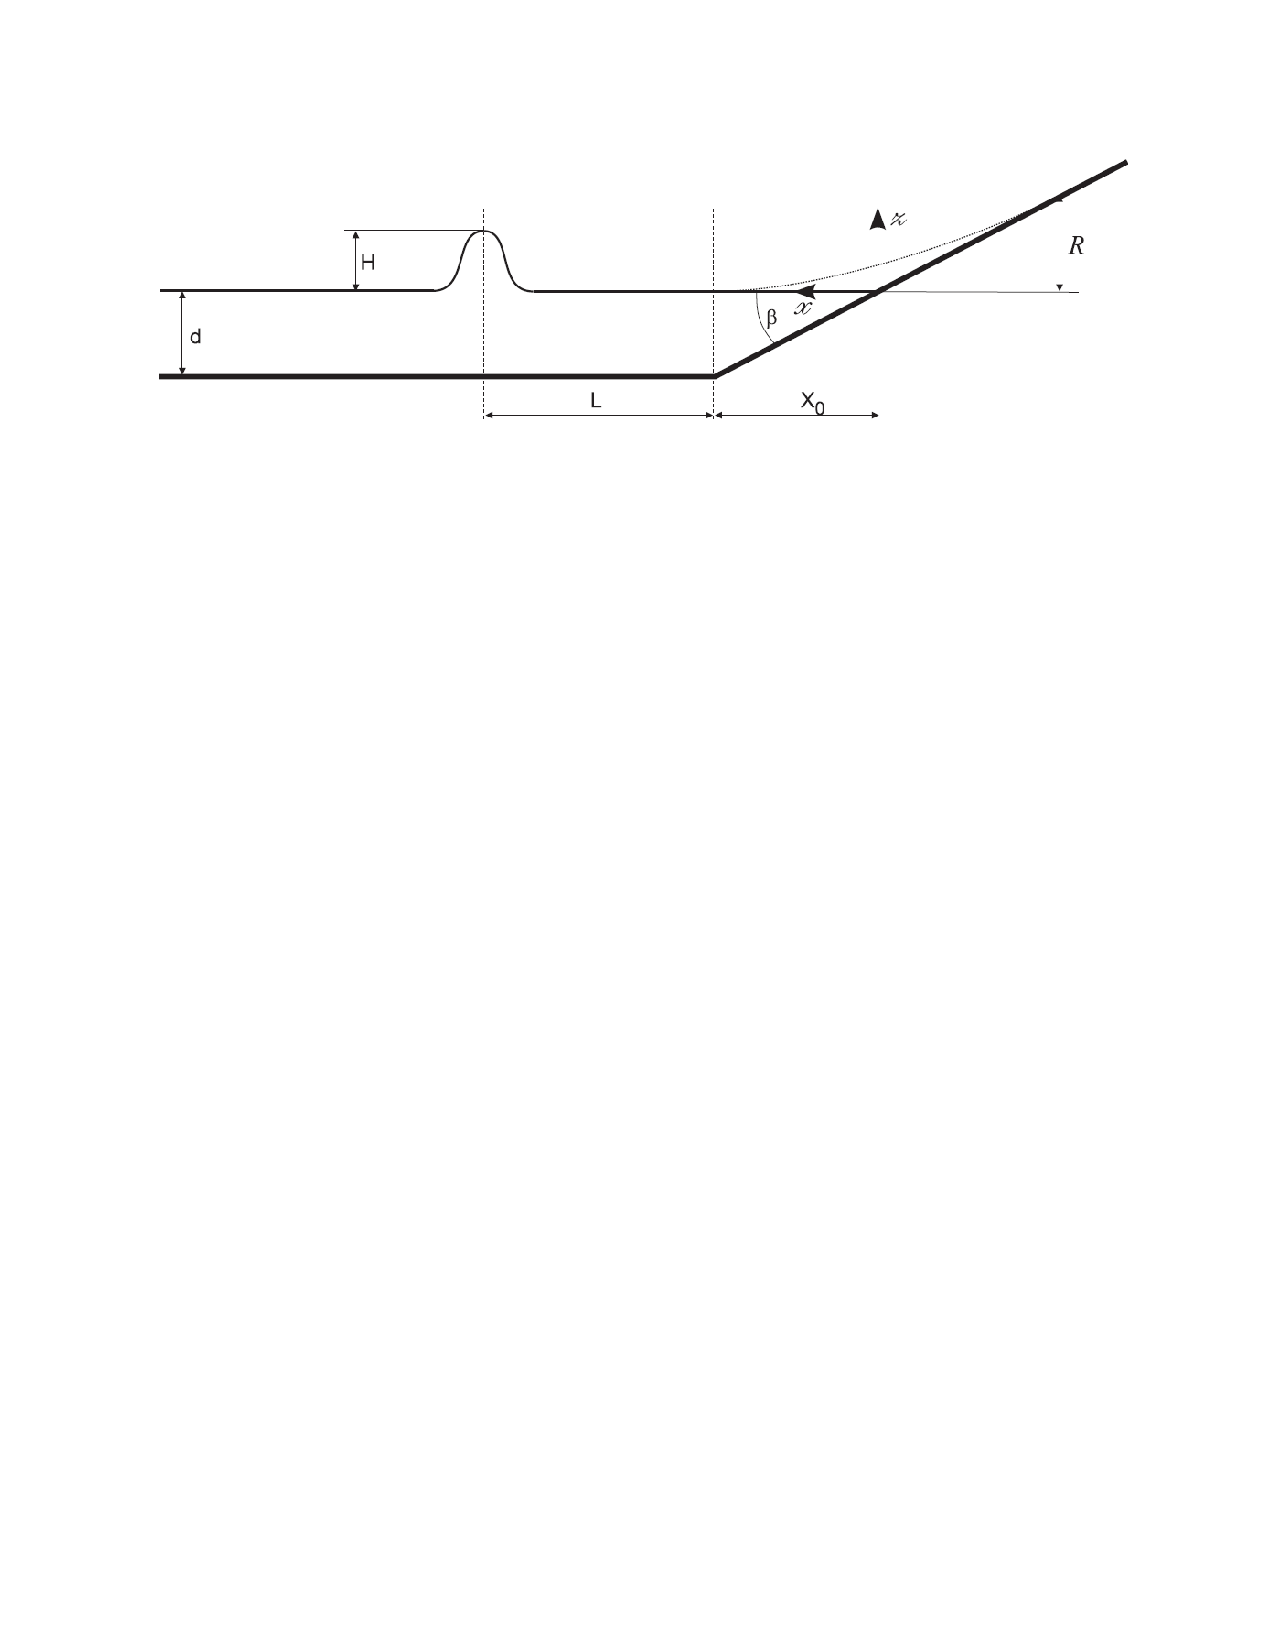
\includegraphics[width=7.0in]{bp4/domainbp4.pdf}\hfil
\caption{\label{domainbp4}
Schematic of computational domain.
  }
\end{figure}

\subsubsection{Tasks}

\begin{itemize}
\item a. Compare numerically calculated surface profiles at t/T=30:10:70 for the non-breaking case H/d=0.0185 with the lab data.
\item b. Compare numerically calculated surface profiles at t/T=15:5:30 for the breaking case H/d=0.3 with the lab data
\item c. (Optional) Demonstrate the scalability of the code by using different d
\item d. Compute maximum runups for at least one non-breaking and one breaking wave case.
\end{itemize}

\subsubsection{Problems encountered}

\begin{itemize}
\item Problems that prevented completion of the benchmark were not encountered.
\end {itemize}

\subsubsection{What we did}

\begin{itemize}
\item Used $g=1$ and no friction.
\item The bathymetry consisted of a deep plateau of constant depth $d$
connected to a sloping beach of angle $\beta = \text{arccot}(19.85)$.
Note that the toe of the beach was located at $x = X_0 = d\, \text{cot} \beta$
\item The initial waveform of the wave was given by 
\begin{equation}
\eta(x,0) = H \text{sech}^2(\gamma (x - X_1)/d)
\end{equation}
where $L = \text{arccosh}(\sqrt(20))/\gamma$, $X_1 = X_0 + L$, 
and $\gamma = \sqrt(3H/4d)$. The speed of the wave is given by: 
\begin{equation}
u(x,0)=-\sqrt{g/d}\eta(x,0)
\end{equation}
\item For the low amplitude case, we set $d = 1$ cm, $H = 0.0185$ cm, and
ran the computations on an $800\times 2$ grid, where the x domain
spanned from $x = -10$ to $x = 60$.
\item For the high amplitude case, we set $d = 1$ cm, $H = 0.3$ cm,
and ran the computations on a $1200\times 2$ grid, where the x domain
spanned from $x = -10$ to $x = 60$.
\item We allowed variable time stepping based on a CFL number of 0.9
\end{itemize} 

\subsubsection{Results}

\begin{itemize}
\item Tasks a and b:
Figures \ref{bp2framesa} and \ref{bp2framesb} present the computed and measured surface profiles for the low and high amplitude cases, respectively.  Correspondence is excellent in the low amplitude case.  In the high amplitude case the computed amplitude is smaller and the steepness greater than that of the measured wave -- a consequence of the fact that the experimental parameters violate the shallow water wave assumptions.
\item Task c: This optional task was not addressed.
\item Task d:  Figures \ref{MaxRunup0185} and \ref{MaxRunup3} present the results for maximum runup computations for the low amplitude and high amplitude wave cases.  The results can be expressed as the non-dimensional data pairs (H/d,R/d) = (0.0185,0.085) and (0.3,0.42) for the high and low amplitude cases, respectively.  The low amplitude result falls well within the scatter plot results of Zhan \cite{bp-description} presented in Figure \ref{bp4maxrscatter}, while the high amplitude result falls somewhat below, as might be expected in light of the comments made in the Task a and b discussion, above.
\end{itemize}

\begin{figure}[ht]
\hfil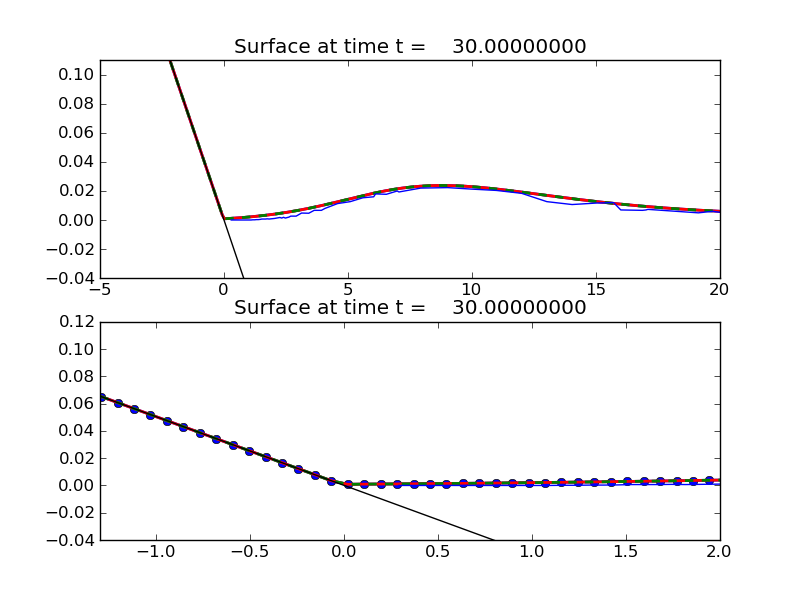
\includegraphics[width=2.8in]{bp4/lab-185/frame0001fig2.png}\hfil
\hfil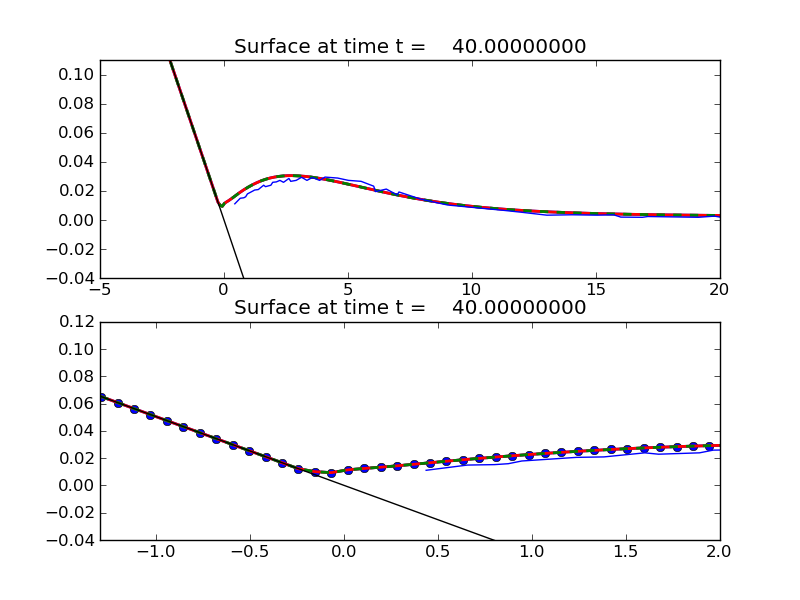
\includegraphics[width=2.8in]{bp4/lab-185/frame0002fig2.png}\hfil
\vskip 5pt
\hfil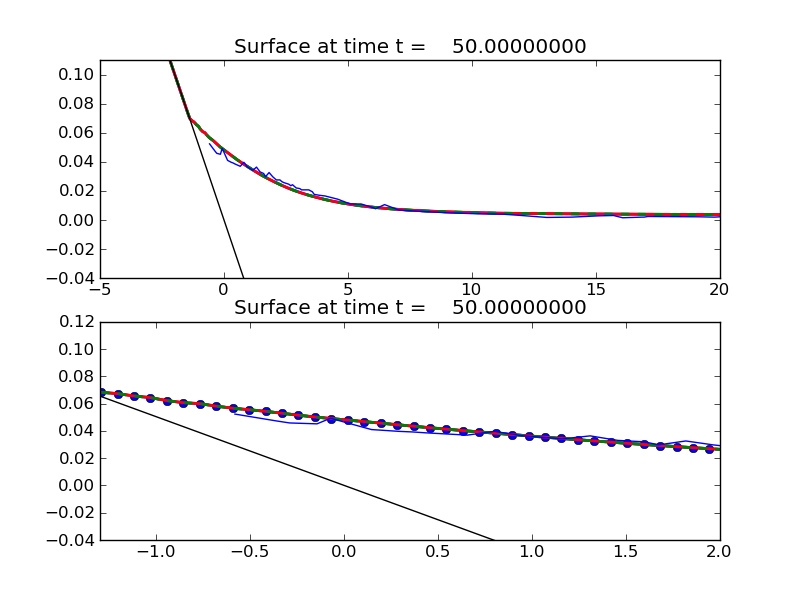
\includegraphics[width=2.8in]{bp4/lab-185/frame0003fig2.png}\hfil
\hfil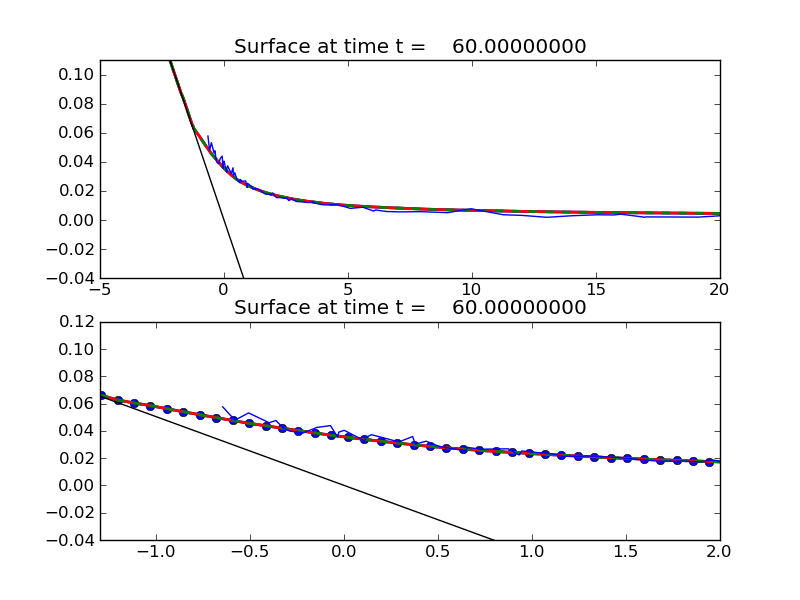
\includegraphics[width=2.8in]{bp4/lab-185/frame0004fig2.png}\hfil
\vskip 5pt
\hfil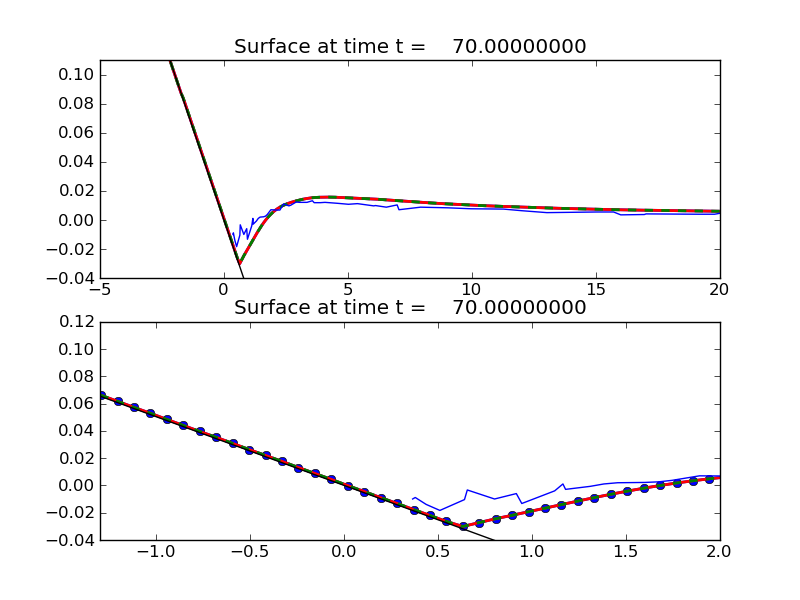
\includegraphics[width=2.8in]{bp4/lab-185/frame0005fig2.png}\hfil
\caption{\label{bp2framesa} 
Runup computations for the low amplitude case. In the paired plots for each time value, the bottom frame provides a zoomed view of the inundation area for the incident wave presented in the top frame.
%\todo{Replot with only two curves?}
}
\end{figure}

\begin{figure}[ht]
\hfil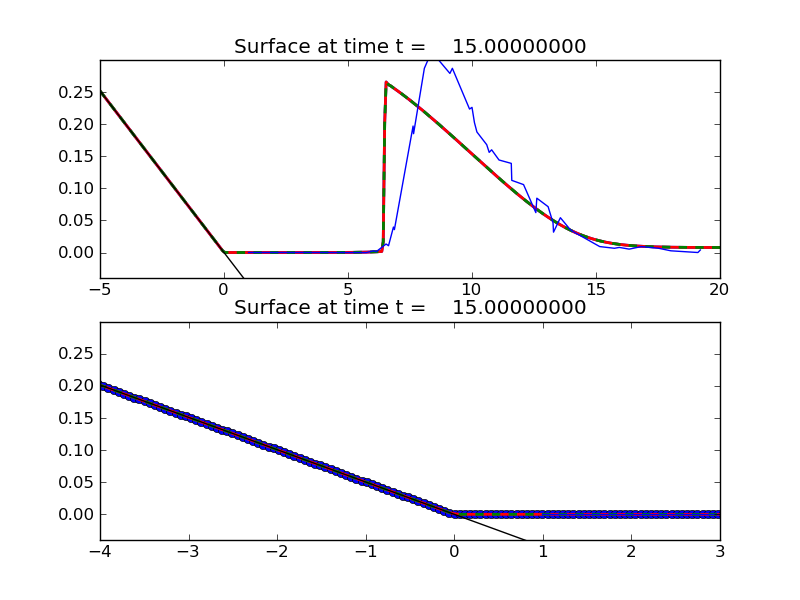
\includegraphics[width=2.8in]{bp4/lab-3/frame0001fig2.png}\hfil
\hfil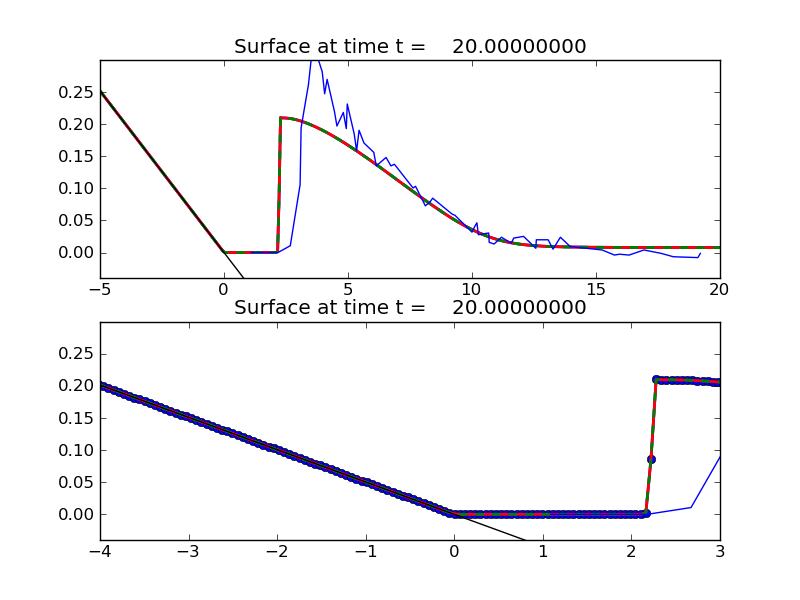
\includegraphics[width=2.8in]{bp4/lab-3/frame0002fig2.png}\hfil
\vskip 5pt
\hfil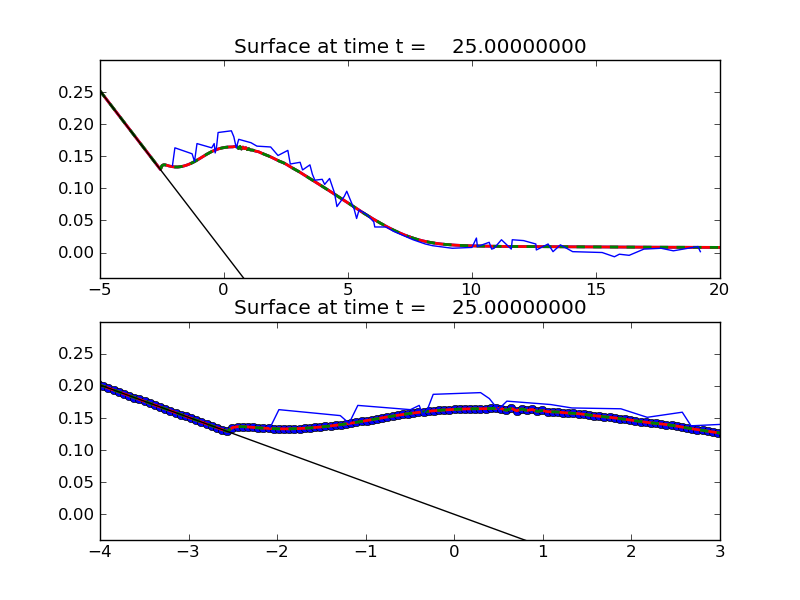
\includegraphics[width=2.8in]{bp4/lab-3/frame0003fig2.png}\hfil
\hfil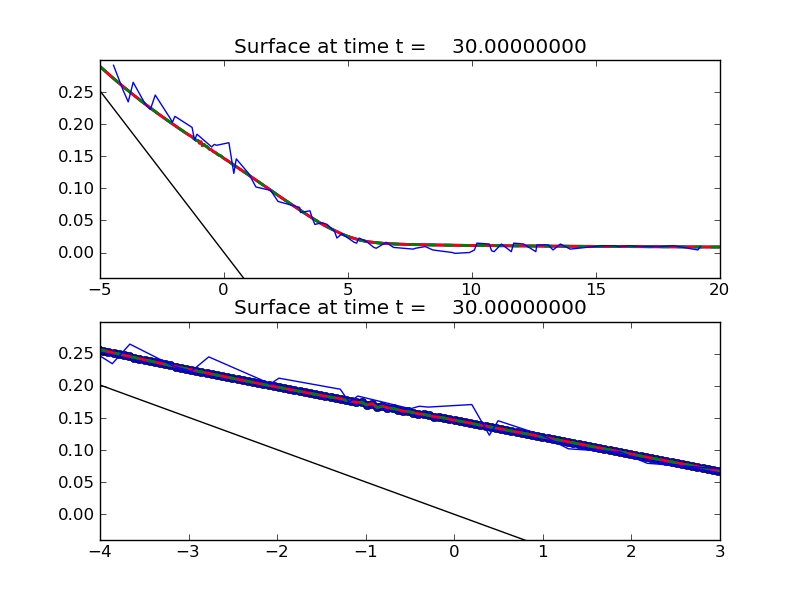
\includegraphics[width=2.8in]{bp4/lab-3/frame0004fig2.png}\hfil
\caption{\label{bp2framesb} 
Runup computations for the high amplitude case. In the paired plots for each time value, the bottom frame provides a zoomed view of the inundation area for the incident wave presented in the top frame.
%\todo{Replot with only two curves?}
}
\end{figure}

\begin{figure}[ht]
\hfil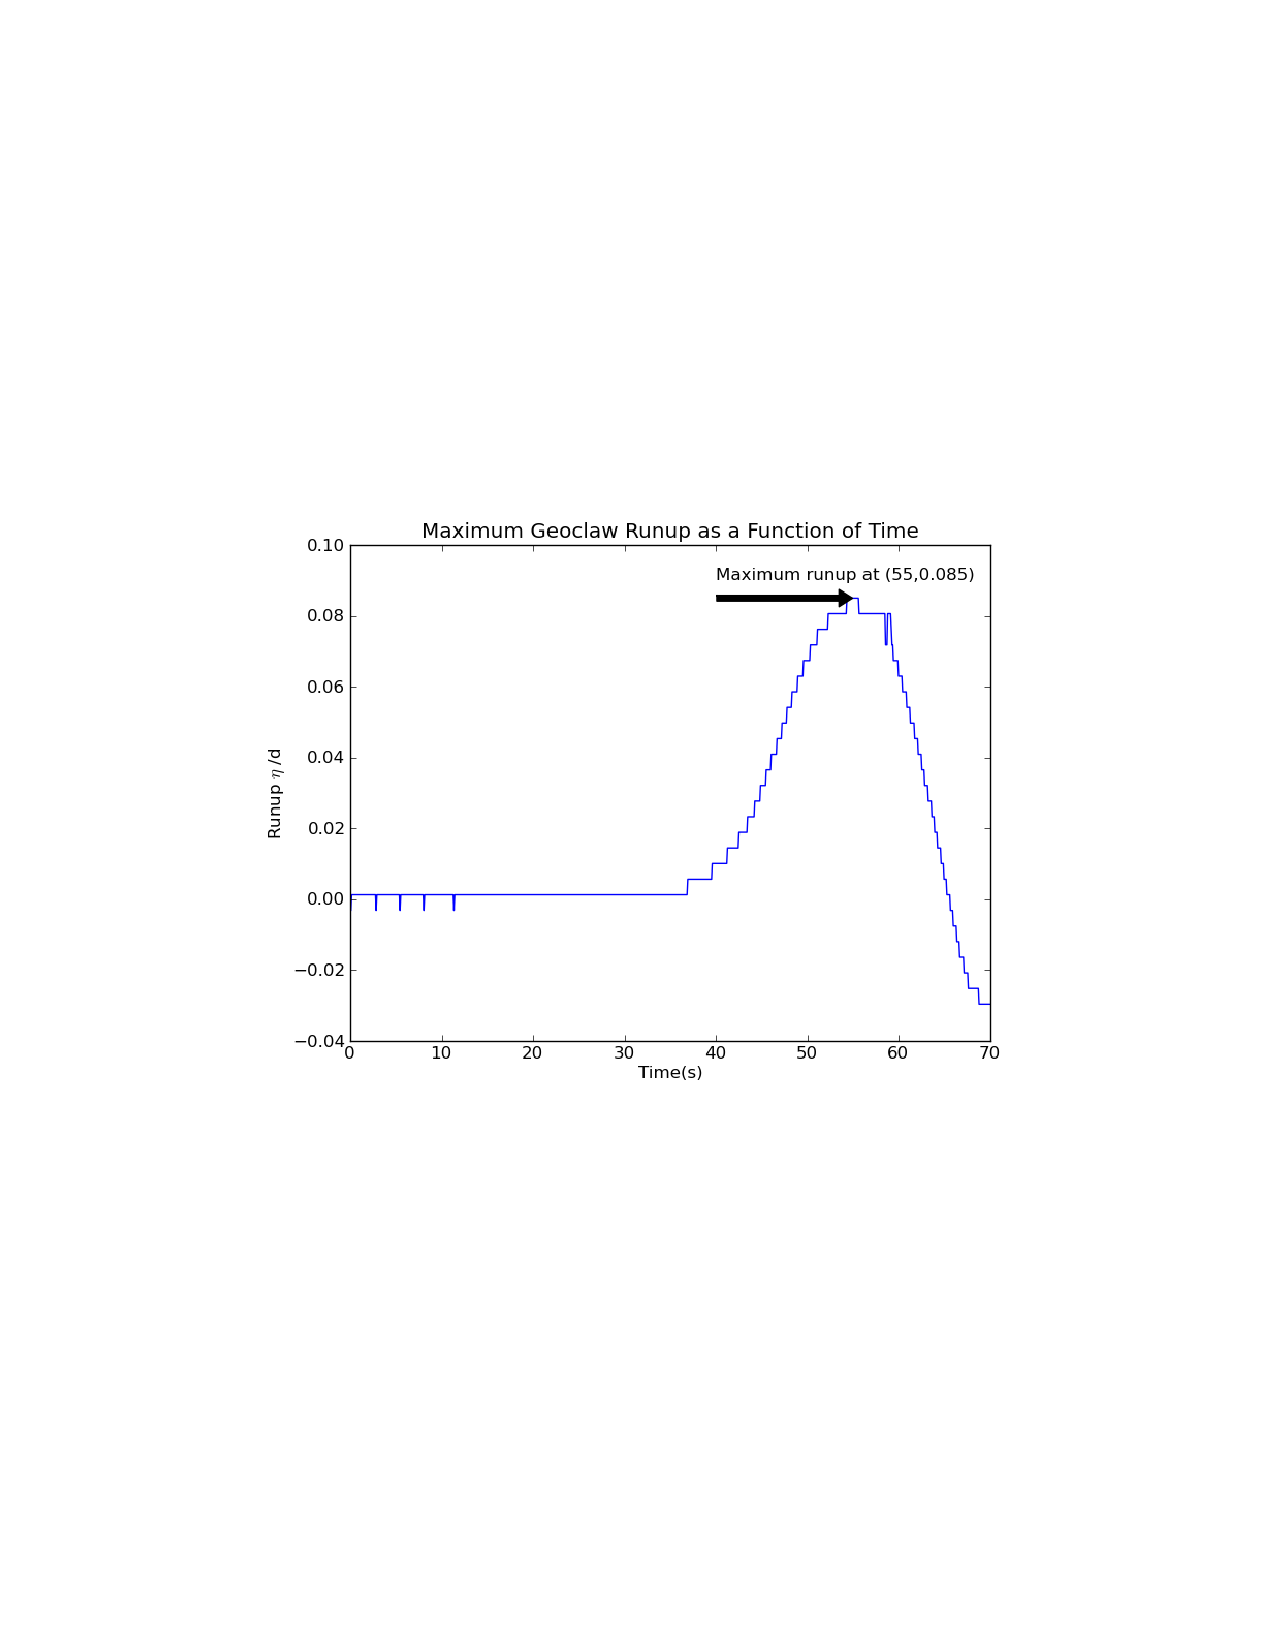
\includegraphics[width=2.8in]{bp4/MaxRunup0185.pdf}\hfil
\caption{\label{MaxRunup0185} 
Maximum runup estimate of 0.085 cm for the low amplitude case, occurring at 55 seconds of the computation. 
}
\end{figure}

\begin{figure}[ht]
\hfil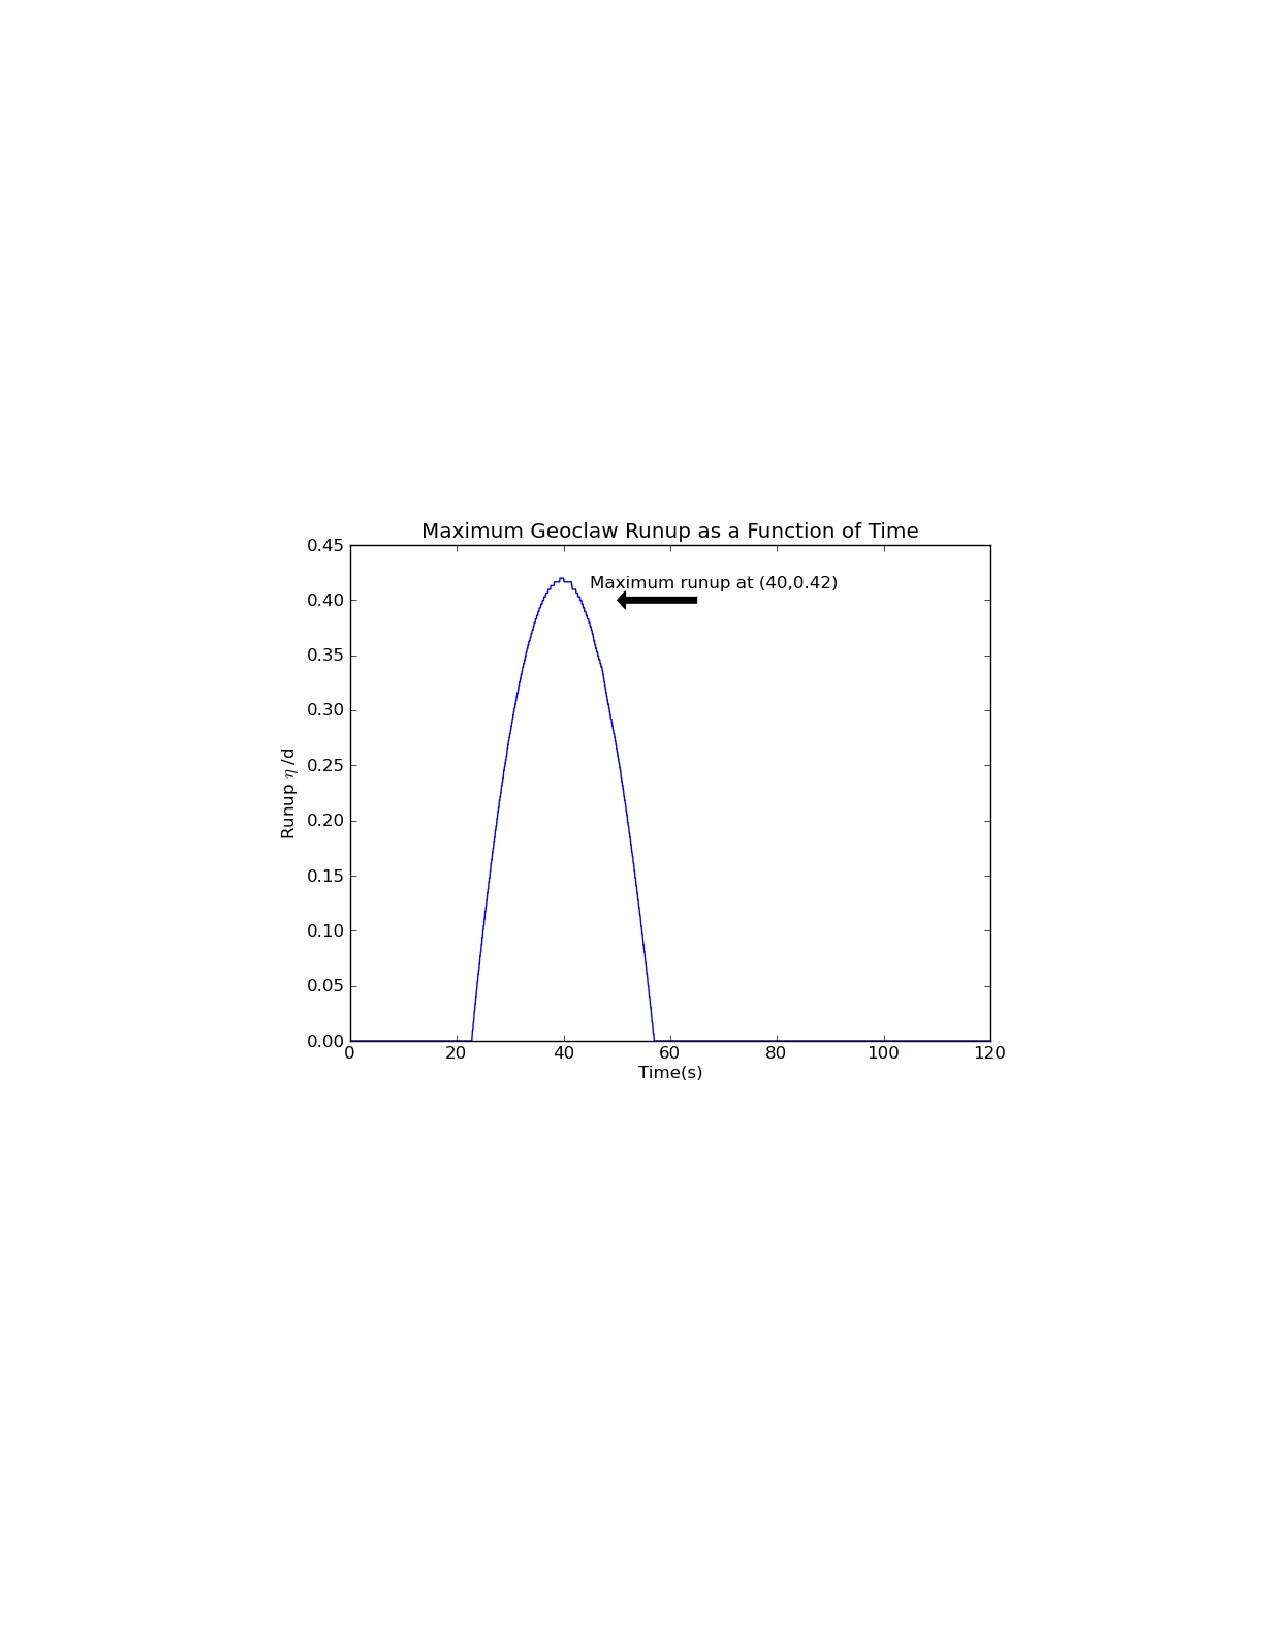
\includegraphics[width=2.8in]{bp4/MaxRunup3.pdf}\hfil
\caption{\label{MaxRunup3} 
Maximum runup estimate of 0.42 cm for the high amplitude case, occurring at 40 seconds of the computation. 
}
\end{figure}

\begin{figure}[ht]
\hfil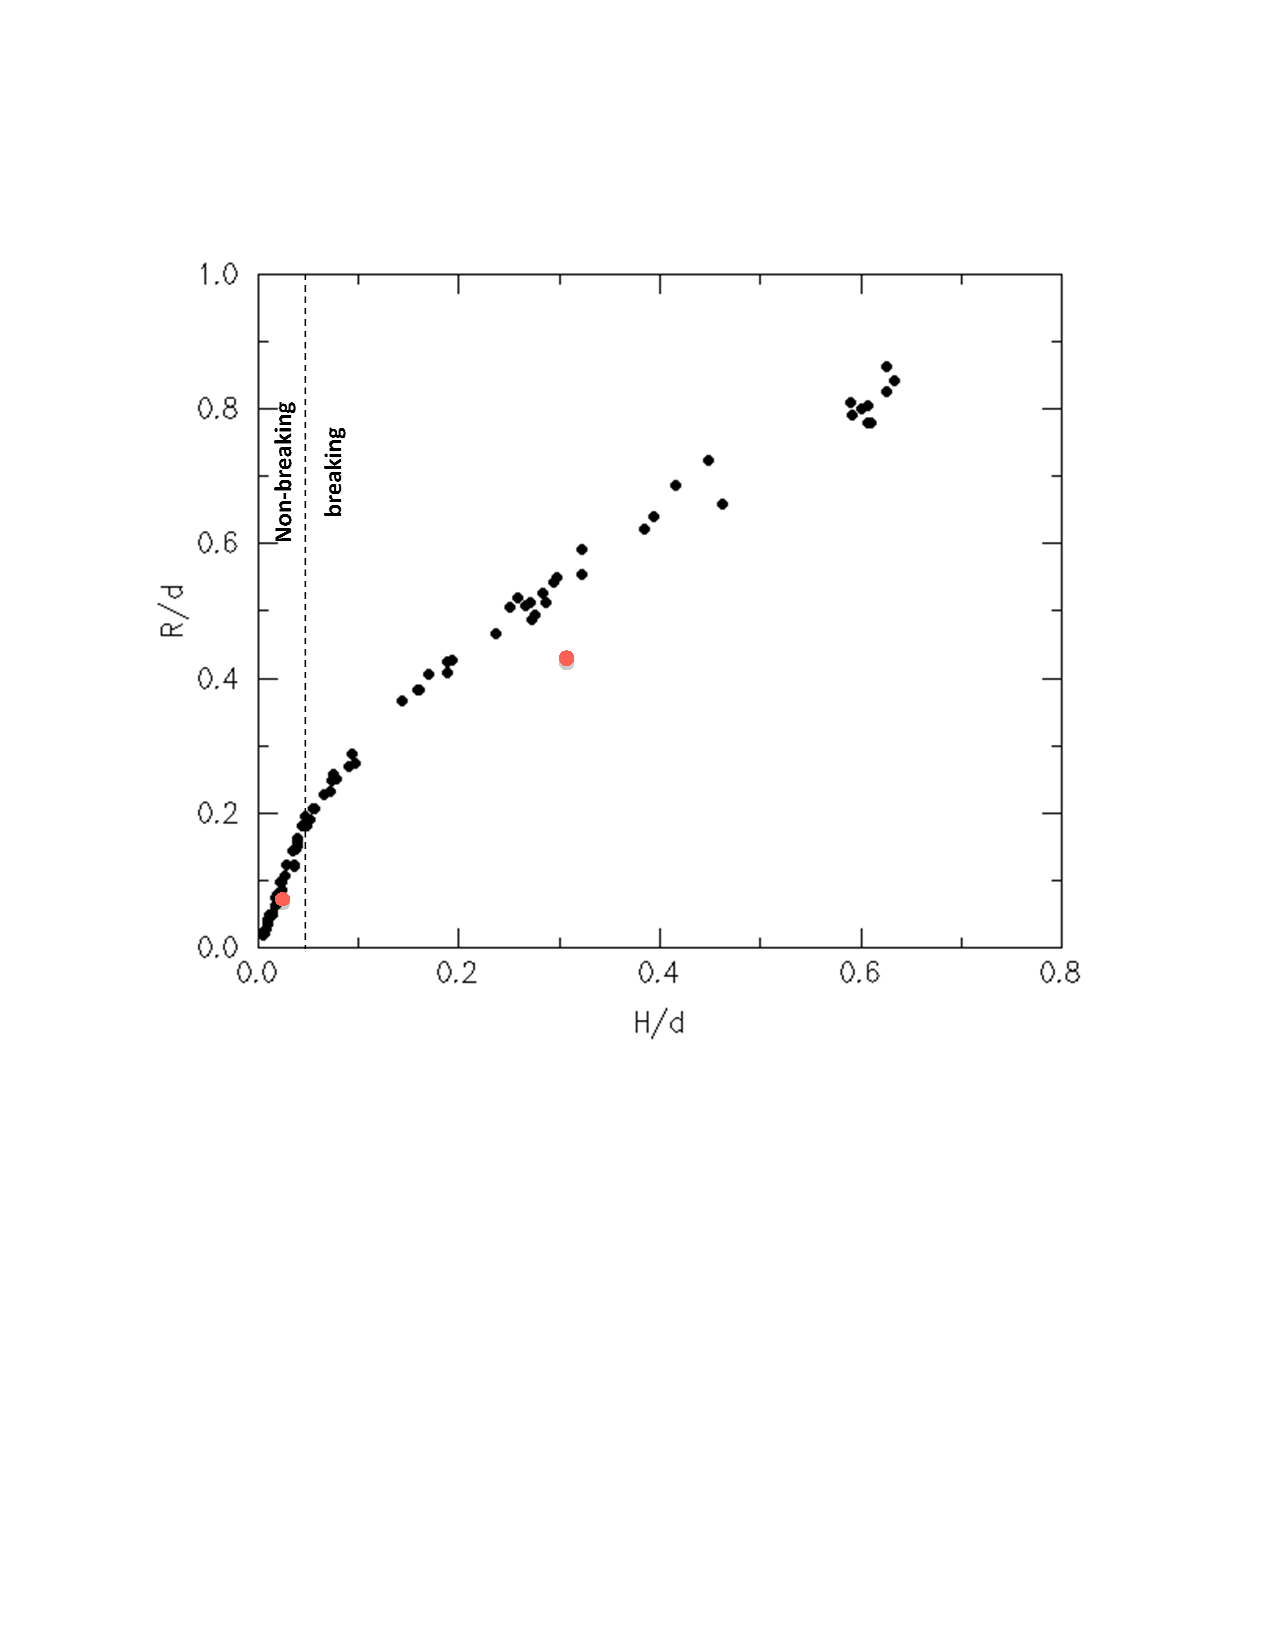
\includegraphics[width=5.0in]{bp4/bp4maxrscatter.pdf}\hfil
\caption{\label{bp4maxrscatter} 
Scatter plot of nondimensional maximum runup, R/d, versus nondimensional incident wave height, H/d, resulting from a total of more than 40 experiments conducted by Y. Joseph Zhan and described at \cite{bp-description}.\\
%\todo{Add points for our two experiments?}
}
\end{figure}

\subsubsection{Lessons learned}

For test cases in which amplitudes are so large that the shallow water wave assumptions are violated, it can be expected that computed and observed wave height and runup will not agree as well as in cases characterized by amplitudes for which the shallow water wave assumptions are valid.

For the high-amplitude $H/d = 0.3$ case, our observed runup of $0.42$
agrees well with the experimental results shown in
Figure~\ref{bp4maxrscatter}.
